\documentclass[titlepage,11pt]{article}
\usepackage[utf8]{inputenc}
\usepackage{fullpage}
\usepackage{indentfirst}
\usepackage[per-mode=symbol]{siunitx}
\usepackage{listings}
\usepackage{graphicx}
\usepackage{color}
\usepackage{amsmath}
\usepackage{array}
\usepackage[hidelinks]{hyperref}
\usepackage[format=plain,font=it]{caption}
\usepackage{subcaption}
\usepackage{standalone}
\usepackage[nottoc]{tocbibind}
\usepackage{scrextend}
\usepackage[margin=1in]{geometry}
\usepackage{lstautodedent}


\definecolor{dkgreen}{rgb}{0,0.6,0}
\definecolor{gray}{rgb}{0.5,0.5,0.5}
\definecolor{mauve}{rgb}{0.58,0,0.82}

\lstset{frame=tb,
  language=Java,
  aboveskip=3mm,
  belowskip=3mm,
  showstringspaces=false,
  columns=flexible,
  basicstyle={\small\ttfamily},
  keywordstyle=\color{blue},
  commentstyle=\color{dkgreen},
  stringstyle=\color{mauve},
  breaklines=true,
  breakatwhitespace=true,
  tabsize=3,
  basicstyle=\scriptsize\tt,
  autodedent,
  numbers=left,
  numberstyle=\tiny\color{gray},
  xleftmargin=2.5em,
  frame=single,
  framexleftmargin=2em
}
% PC
%\def \espath {"C:/Users/Sean/IdeaProjects/Prometheus/src/es/ExpertSystem.java"}
%\def \knnpath {"C:/Users/Sean/IdeaProjects/Prometheus/src/knn/KnowledgeNodeNetwork.java"}

% OSX
\def \espath {"/Users/seanstappas1/GitHub/prometheus-ai/es/ExpertSystem.java"}
\def \knnpath {"/Users/seanstappas1/GitHub/prometheus-ai/knn/KnowledgeNodeNetwork.java"}

\def\equationautorefname~#1\null{%
  Equation~(#1)\null
}

\def\sectionautorefname~#1\null{%
  Section~#1\null
}

\def\subsectionautorefname~#1\null{%
  Subsection~#1\null
}

\def\arraystretch{1.3}%  1 is the default, change whatever you need

% Custom commands
\newcommand{\ar}[1]{\autoref{#1}}
\newcommand\numberthis{\addtocounter{equation}{1}\tag{\theequation}}
\newcolumntype{P}[1]{>{\centering\arraybackslash}p{#1}}
\newcommand{\code}[1]{\texttt{#1}}
\newcommand{\specialcell}[2][c]{%
	\begin{tabular}[#1]{@{}c@{}}#2\end{tabular}}

\title
{
	\uppercase{Prometheus AI} \\
	\large Phase 1
}
\author % (optional, for multiple authors)
{
	Sean Stappas \\ 
	260639512 \\
	\\ 
	ECSE-498: Honours Thesis I \\
	\\
	\small Supervised by: Prof. Joseph Vybihal
}
\date{April 11, 2017}

\begin{document}
	
\sloppy

\maketitle

\section*{Abstract}
% The abstract is an executive summary of your project/thesis. It should provide an overview of your project/thesis by addressing the following questions. a. What is the motivation for the project/thesis? b. What are the goals of the project/thesis? c. What was achieved this semester? d. What methods were used to make those achievements? The abstract should be between 200 and 250 words long.
Prometheus AI is a model of the human brain with the goal of controlling multiple robots in a swarm environment. This could be useful in environments hazardous for humans, such as the aftermath of a nuclear power disaster, or in outer space. The model consists of four layers: the Neural Network (NN), the Knowledge Node Network (KNN), the Expert System (ES), and the Meta Reasoner (META). The NN classifies the signals coming from the robots' sensors and sends formatted tags to the KNN. The KNN represents memory and can initiate cascaded activation of memories in the form of tags, which are passed on to the ES. The ES is a simple logic reasoner and provides recommendations for actions to the META. The META represents high-level thinking and makes an intelligent decision for what the robots should do. The assigned task this semester was to implement prototypes of the KNN and ES layers in Java. This was achieved using specific design criteria and extensive feedback from the project supervisor, Prof. Vybihal. Personal design criteria included using object-oriented programming principles, optimizing the system for speed and space efficiency, and maximizing code readability. Tests were created in TestNG and extensive documentation was written in Javadoc.

\section*{Acknowledgments}
% If applicable, you may acknowledge people here who contributed to the project in some way but are not listed on the title page. (For example, if you received advice, data, or supervision from graduate students or others.)
Elsa Riachi worked on the other two layers of the Prometheus AI (NN and META) in parallel with the work done in this report. She is also doing this project as part of an Honours Thesis. Many discussions were had together on the design of the system and how the layers should fit together.

\clearpage
\tableofcontents

\listoffigures
\listoftables
\lstlistoflistings
\clearpage

\twocolumn

\section*{Abbreviations}
% List of abbreviations and/or notation used in the report.

The following abbreviations will be used throughout the report:

\begin{labeling}{abbreviations}
\item [NN] Neural Network.
\item [KNN] Knowledge Node Network.
\item [KN] Knowledge Node.
\item [ES] Expert System.
\item [META] Meta Reasoner.
\item [OOP] Object-Oriented Programming.
\end{labeling}

\section{Introduction} \label{sec:intro}
% In this section you should introduce (at a high level) the overall theme of the project, and state clearly what are the goals you are trying to achieve.  This section should also clearly convey why this project is important, what is the potential impact (applications, etc).

The goal of this project is to create an artificial intelligence system to control multiple robots. Applications for this type of system include robots in hazardous environments, such as in outer space (Mars, Moon, etc.), in nuclear plants after a nuclear disaster, and in military zones.

The robots themselves are expected to have a fixed front-facing camera and ultrasonic sensor(s). Each robot may have multiple fixed ultrasonic sensors pointing in different directions, or a single rotating ultrasonic sensor that sweeps the area in front of the robot. The ultrasonic sensor(s) can measure distance between the robot and nearby objects, and the camera can take images of what the robot is facing.

The structure of the system is inspired from the functionality of the human brain, and is composed of the following four layers (in order of increasing abstraction): the Neural Network (NN), the Knowledge Node Network (KNN), the Expert System (ES), and the Meta Reasoner (META) \cite{vybihal-model}. The system can be seen in \autoref{model} and will be described in \autoref{sec:background}.

\begin{figure}[!htb]
	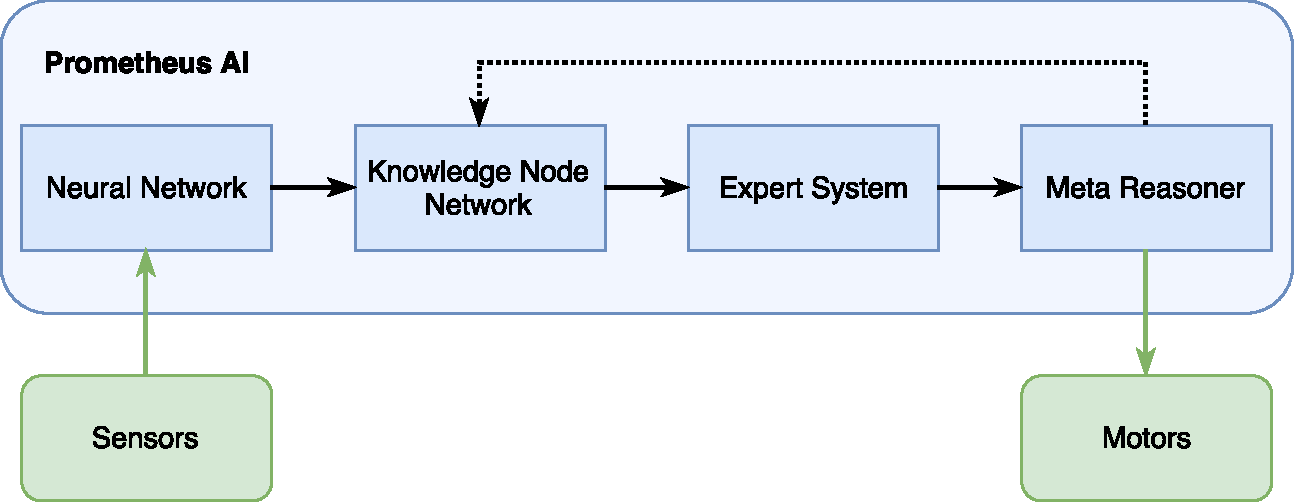
\includegraphics[width=\columnwidth]{figures/ai_model.pdf}
	\caption{Prometheus AI model.}
	\label{model}
\end{figure}

\section{Background}
\label{sec:background}
% In this section you should summarize the theory and background that you had to learn, and that you believe are necessary for the reader to understand the rest of the report.

\subsection{Neural Network}

The NN layer consists of a network of neurons with a similar structure to neurons in the human brain. In the context of this project, it is the interface between the robots' sensors (camera and ultrasonic) and the rest of the AI system.

The NN gathers raw sensor data and will build an abstract view of the robot's surrounding environment. It will analyze the contents of the camera image and achieve two main goals:

\begin{enumerate}
	\item Classify objects observed in the image.
	\item Localize objects in the image.
\end{enumerate}

To achieve these goals, a convolutional neural network will be used, which can determine which regions of the image are important and classify objects in those regions \cite{conv}. A 3D view of the world will also be generated. Using ultrasonic sensor readings and coordinate transformations from the world to the camera images, the observed objects can be localized in space.

Ultimately, the classification and localization of objects will produce abstract informational tags, which will be passed on to the KNN. These tags can therefore be measures of the position of an object, or other characteristics about an object.

\subsection{Knowledge Node Network}

The KNN layer represents memory in the human brain. It takes in the tags provided by the NN and outputs tags based on its knowledge of the environment. The KNN is based around interconnected Knowledge Nodes (KNs), which are abstract structures representing memories and their connections to other memories. A simple model of a Knowledge Node (KN) can be seen in \ar{kn}.

\begin{figure}[!htb]
	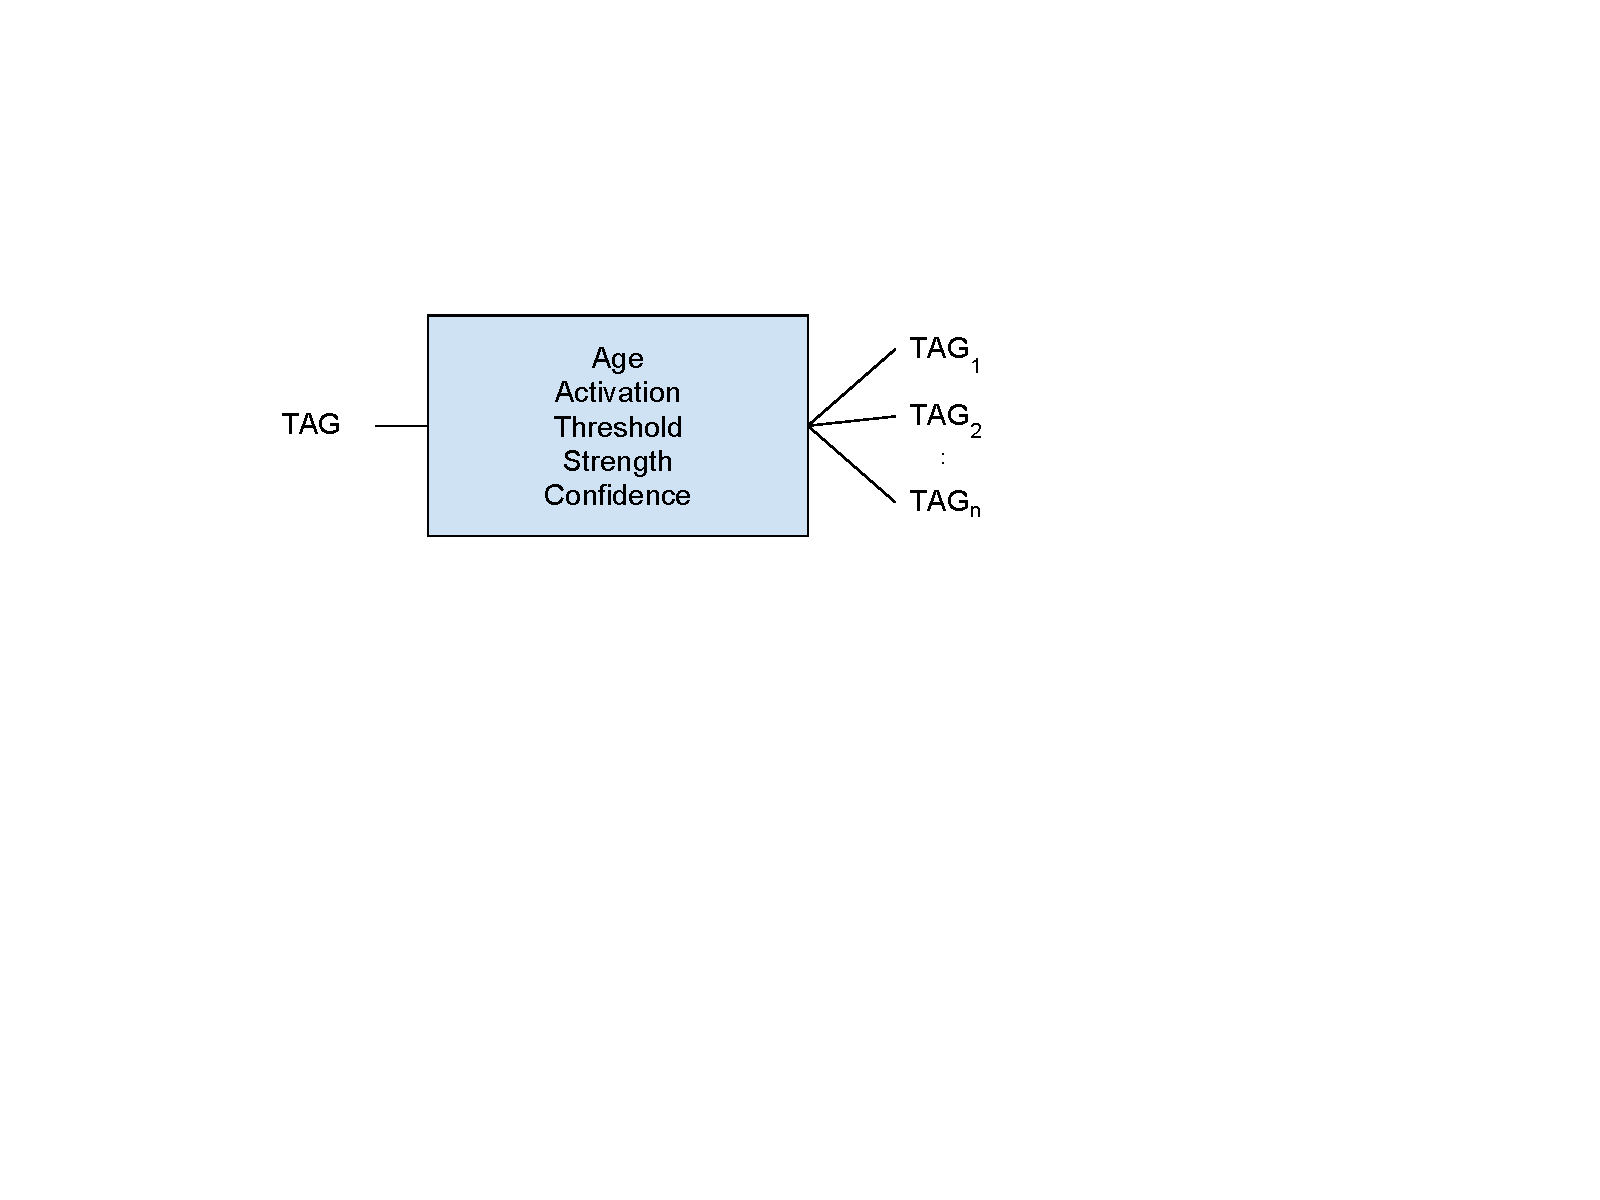
\includegraphics[width=\columnwidth]{figures/kn.pdf}
	\caption[High-level model of the Knowledge Node of the KNN.]
	{High-level model of the Knowledge Node (KN) of the KNN \cite{vybihal-knowledge}.}
	\label{kn}
\end{figure}

KNs have an input tag representing some information, and output tags representing information related to the input tag. Tags in the KNN can become ``active'', meaning that they are observed or seen as true. For example, if the NN determines that it observes a ball and passes that information on to the KNN, then a ``ball'' tag may become active in the KNN. This would excite the KN with input tag ``ball''. If that KN fires, other tags related to that observation can become active. For example, tags representing ball characteristics such as ``round object'' may become active. This tag in turn may be connected to another KN, potentially causing more activation.

There are different ways that KN excitation could be implemented. With simple linear activation, an excitation would increment the node's activation parameter, which initially starts at 0. If $activation \geq threshold$, the KN fires, causing the activation of the output tags. This description corresponds to forwards thinking. The activation can also be with a sigmoid function, which is more representative of neurons in the brain \cite{neuro}.

% TODO: talk more about relation to neurons in brain, and ways to leverage this

There is a strength value associated with every KN which represents how much weight an activation has and therefore how quickly that node will fire. A simple implementation of strength would be as a constant coefficient multiplying the activation parameter. So, instead of checking when the activation is greater than the threshold, one would check if $activation * strength \geq threshold$, where the strength is positive. The strength value could be 0 however, which effectively shuts off the KN. Another way of implementing strength is to check $activation + strength \geq threshold$. In this case, strength can be negative and hinder the firing of the node.

Strength can be seen as the firing predisposition of neurons in the brain as a result of learning \cite{vybihal-knowledge}. Indeed, learning can increase the synaptic strength between neurons and cause early or late firing of those neurons \cite{hebb}. For example, a person who has had a bad experience with spiders would fire their fear response upon seeing a spider more quickly than one without that fear.

Every KN can have a confidence value associated with it, representing how certain the KNN is that the input tag is true. In this case, the confidence value would be stored within the KN itself. These confidence values can come from the NN, since a neural network will always have a confidence value when classifying objects. When initiating a think cycle, the confidence value at each stage can be multiplied with each other to produce a new confidence value, making the KNN less certain of a memory as it searches through its tree of KNs. This represents how belief changes when thinking. Indeed, some memories in the human brain require a great deal of thinking to reach and, as such, can be less certain than other memories. This can lead to the recollection of false memories \cite{falsememories}. % TODO: source (neural network always has confidence value)

Age represents how long it has been since a KN has been excited. The idea is that, after a KN has aged a certain amount of time, that node will be discarded, similarly to how old memories are discarded in the brain \cite{aging}. The intuitive implementation of aging is to constantly increment some age value associated with every KN, and discard nodes whose age is greater than some threshold. The age would be reset when the node is excited. This would however be unnecessarily computationally intensive, requiring some kind of constant updating of every single node. A more efficient way of doing it would be to save a timestamp for every KN when it is excited, and if the KNN attempts to excite a KN whose previous timestamp value is too far into the past, that node is instead deleted.

Thinking in the KNN represents an activation routine, which activates tags and potentially fires KNs. The KNN has three main ways of thinking: forwards, backwards, and lambda. The version of thinking to be done by the KNN is chosen by the META.

Forwards thinking is the simplest and is depicted in \autoref{think_forwards}. Firing a KN can cause forward activation of more KNs, hence the ``forwards'' naming.

\begin{figure}[!htb]
	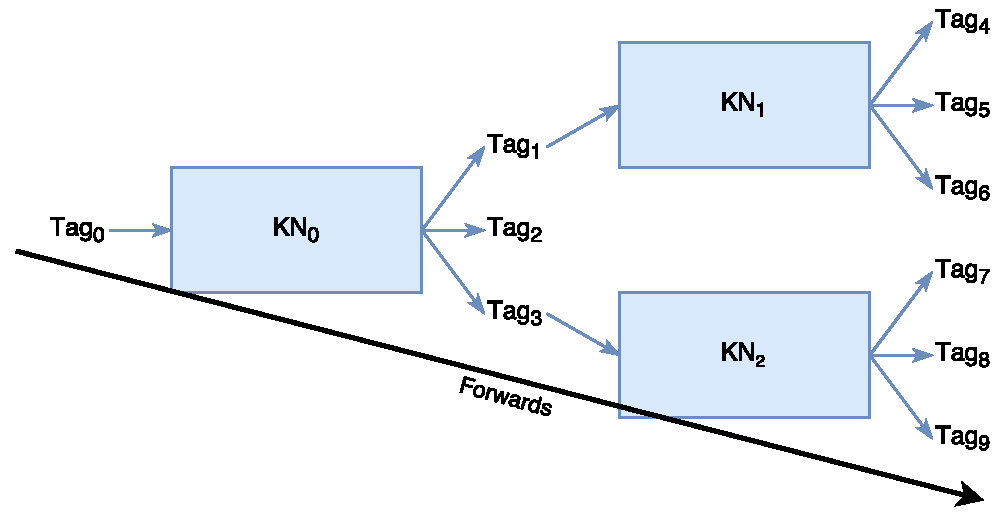
\includegraphics[width=\columnwidth]{figures/forwards_thinking.pdf}
	\caption{Thinking forwards in the KNN.}
	\label{think_forwards}
\end{figure}

Thinking backwards starts at the output tags of KNs, and works backwards, as can seen in \autoref{think_backwards}. In its simplest form, it checks output tags of KNs and, if all of them are active, the input tag must be active as well, so that KN is fired.

\begin{figure}[!htb]
	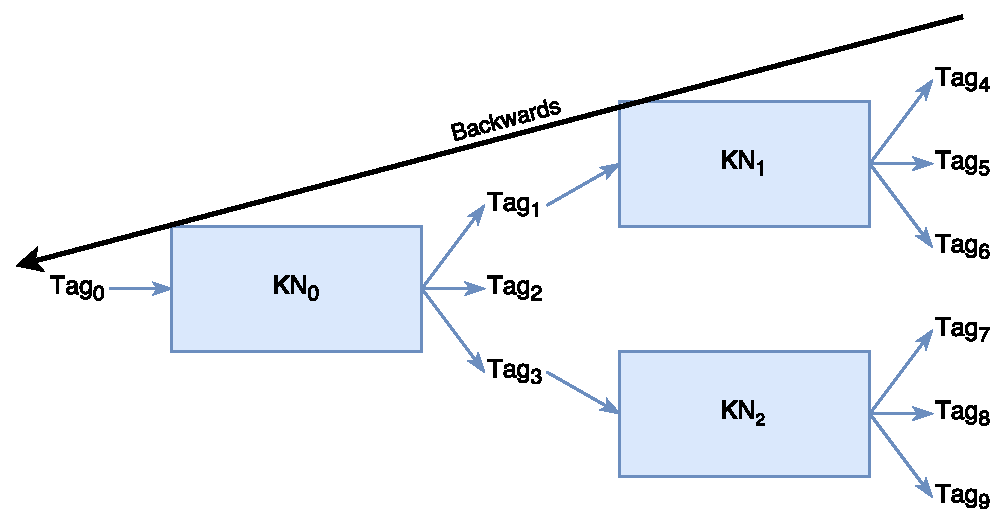
\includegraphics[width=\columnwidth]{figures/backwards_thinking.pdf}
	\caption{Thinking backwards in the KNN.}
	\label{think_backwards}
\end{figure}

This type of thinking can be more difficult to implement than forwards thinking, since one must decide what percentage of active output tags of a KN corresponds to an active input tag. For instance, should a KN fire when 100\% of its output nodes are active, or when 75\% are active? This relates to the confidence with which the KNN believes the tag associated with that node to be true. As a concrete example, if you observe an object that has four wheels, seats, and a steering wheel, how confident are you that that object is a car? Realistically, humans with often classify what they observe with some uncertainty \cite{uncertainty} and this is what can be represented with backwards thinking. This type of thinking occurs constantly in the background in humans \cite{vybihal-knowledge}, and this is something to keep in mind during implementation.

Lambda thinking uses a combination of forwards and backwards, and can be seen in \autoref{think_lambda}. It is called ``lambda'' thinking because the shape of the thinking trajectory matches a Greek uppercase lambda ($\Lambda$). It first looks at output tags of KNs and propagates activation backwards, similar to backwards thinking. After a certain amount of nodes are fired, it will then start activating forwards, similar to thinking forwards. An interesting question is how far backwards should lambda thinking go before starting to cascade forwards? This relates to how general one wants to explore before searching for a more specific value.

\begin{figure}[!htb]
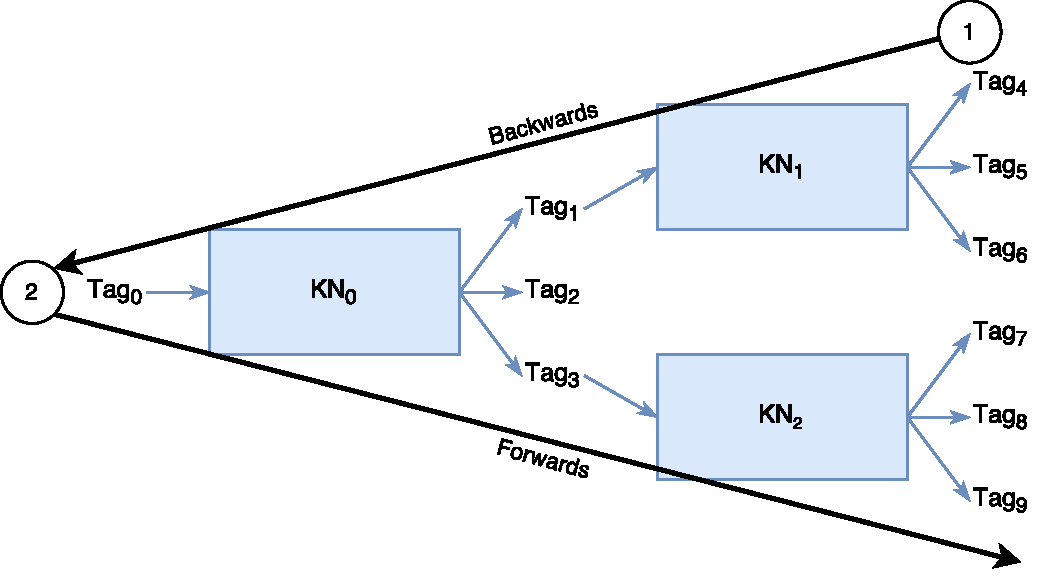
\includegraphics[width=\columnwidth]{figures/lambda_thinking.pdf}
\caption{Lambda thinking in the KNN.}
\label{think_lambda}
\end{figure}

This type of thinking occurs in humans when using analogical reasoning to find a memory \cite{vybihal-lambda}. In essence, when a person wants to locate a memory that is not directly accessible, they will explore related memories, move their way ``backwards'' to concepts related to the desired memory, and think ``forwards'' to focus in on the desired memory. For example, if one is asked where they were in 2002 at a specific date, they most likely would not remember. If they explore related dates and events in their life, however, they may be able to narrow down and extract that memory. In the context of the Prometheus system, lambda thinking will be attempted if all other forms of thinking fail (forwards and backwards).

All forms of thinking can continue until there are no more KNs to activate, which corresponds to natural quiescence. There can also be a fixed number of thinking cycles, which represents how much effort is being put into thinking. Indeed, in humans, thinking is done with varying degrees of effort \cite{thinking}, and it would be interesting to model this.

The result of all forms of thinking is a collection of activated tags, which are passed on to the ES.

\subsection{Expert System}

The ES layer is a basic logic reasoner. It is not aware of its current reality or any context. It takes in the tags provided by the KNN and interprets them as either facts, recommendations or rules.

Facts are simple calculus predicates showing that something is true. Here are some examples of fact tags and their meanings:

\begin{labeling}{$(A > 1)$}
	\item[$(A)$] $A$ itself is true or active.
	\item[$(A = 1)$] $A$ is equal to 1.
	\item[$(A > 1)$] $A$ is greater than 1.
	\item[$(A \ ?)$] $A$ can take any value.
\end{labeling}

As a more concrete example, a fact can represent a certain measurement, like $(distance = 5)$ representing the robot's distance from a wall as measured by one of its sensors.

Recommendations represent suggestions for actions to be taken by a robot. For example, $(\#turn\_left)$ is a recommendation for a robot to turn left, if it sees a wall directly in front of it and must avoid it, for example. These are recommendations and not commands because the META can decide whether or not to actually take that action.

Rules are many-to-many structures with facts as inputs and recommendations or facts as outputs. This can be seen in \autoref{eq:rule}, where $m \geq 1$ and $n \geq 1$, i.e., there must be at least one input tag and one output tag. 

\begin{equation} \label{eq:rule}
Fact_1 \cdots Fact_m \rightarrow Tag_1 \cdots Tag_n
\end{equation}

When all the input tags become active, the output tags become active and the rule itself is also said to be active. In this way, a rule can represent a logical AND of all its input tags. The runtime of the ES consists of the following general steps \cite{vybihal-expert}:

\begin{enumerate}
	\item Reset.
	\item Add facts and rules.
	\item Think.
	\item Send recommendations to META.
\end{enumerate}

The most important part of the previous process is the thinking stage, which represents the activation routine of the ES. This consists of first iterating through all the rules in the ES and checking if they are active by inspecting the lists of facts and recommendations. Rules may then become active and cause cascading activation of more rules. This can continue until there are no more rules to activate, which corresponds to natural quiescence. There can also be a fixed number of thinking cycles, which represents the effort put into thinking, similarly to the KNN.

The recommendations activated as a result of thinking are passed on to the final layer, the META.

\subsection{Meta Reasoner}

The META layer represents high-level reasoning in human brains. It is aware of its environment and context, and makes decisions based on what it believes to be right. It is paranoid, and constantly checks whether the tags reported by the rest of the AI system make sense based on its expected view of the world. If it decides to make a decision, it sends a command to the actuators of the robots to decide how to move. If it is not happy with the recommendation(s) from the ES, it may initiate another think cycle in the KNN to generate new recommendations(s).

\begin{figure*}[!htb]
	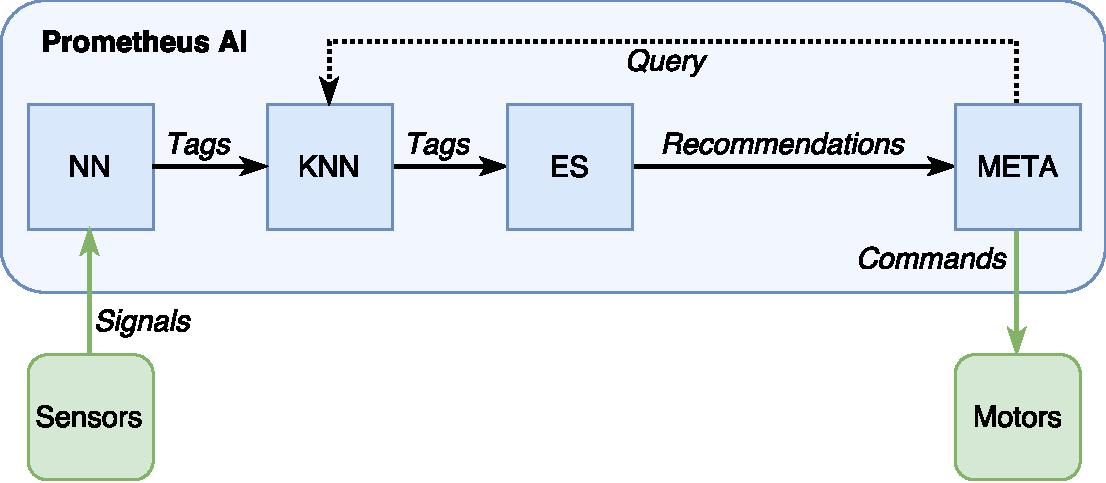
\includegraphics[width=\textwidth]{figures/ai_model_labeled.pdf}
	\caption{Prometheus AI model with labeled input and output.}
	\label{model_labeled}
\end{figure*}

\subsection{Summary}

With this full description of the Prometheus AI model, the system with labeled input and output can be seen in \autoref{model_labeled}.

\section{Problem}
% In this section you should describe the problem or system you are addressing in detail. Describe the project requirements and constraints.

The assigned task was to construct two out of the four layers listed in \autoref{sec:background}: the ES and the KNN. The other two layers are to be completed by another Honours Thesis student.

As a deliverable for the end of this first semester, it was required to complete a prototype of these two layers, with basic versions of the functionality described in \autoref{sec:background}. This was to be done entirely in Java.

\section{Design Criteria}
% In this section you must describe any design work that was already completed. Discuss any design decisions that have been made, and describe the process that was followed to make these decisions. Also discuss any results that have already been obtained this semester.

\subsection{Efficiency}

A very important consideration when designing the system is speed. Since the robots may have to react very quickly to stimuli in the environment, the reasoning in the AI must be as fast as possible. This is especially true in the hazardous environments for which this system could be useful for, as specified in \autoref{sec:intro}. An example of a design choice that was made to improve speed is the use of Java \code{Sets} for most of the collections in the ES and KNN layers. The original specifications mentioned using \code{ArrayLists}, but, since there is no specific iteration order necessary for most operations in the ES and KNN, these collections were changed to \code{HashSets}. This is faster because \code{HashSets} have $O(1)$ access time, whereas \code{ArrayLists} have $O(N)$ access time, where N is the number of elements in the collection. \code{HashSets} also have the advantage of only permitting unique elements.

\subsection{Object Oriented Design}

Another important choice is to leverage object-oriented design as much as possible. Object-oriented programming (OOP) allows extensive planning before even beginning to write code, which can identify any flaws in the initial design. It also allows the code to be very clean and reusable \cite{oop}. Since Java is the programming language chosen for the project, OOP is also the natural way to proceed. To follow OOP, the ES and KNN will be designed around Java classes and the methods associated with those classes. OOP principles such as polymorphism and encapsulation will be followed closely.

\subsubsection{Abstraction}

One important design aspect is that the system should be as abstract as possible, while still performing its desired task. For instance, the system should be general enough to perform under simulations, as well as in real-life environments. It should also ideally be able to perform in vastly different environments, with different tasks.

One example of making use of abstraction is the choice to create a \code{PrometheusLayer} interface for both the ES and KNN, since they share some functionality, like the ability to think.

\subsubsection{Encapsulation}

Each layer of the system has unique, localized functionality that does not need to be visible from the rest of the system. For instance, the intricacies of the \code{think()} method in the ES and KNN layers do not need to be known to the rest of the system.

\subsubsection{Polymorphism}

Many methods in the system can have different functionality depending on context. For instance, the \code{think()} method in the KNN and ES layers can take an optional number of think cycles to specify a threshold for quiescence.

\subsubsection{Inheritance}

Careful thought was put into how objects may inherit functionality from each other. This can most clearly be seen with the implementation of the tags, which will be described in \autoref{sec:implementation}.

\section{Implementation}
\label{sec:implementation}

The details of how the prototype of the system was implemented in Java will now be discussed.

\subsection{Tags}

As described in \autoref{sec:background}, the entire system revolves around tags passed from layer to layer. For this reason, a lot of thought was put into the proper design of these tags.

The tags need to be as general as possible. A natural choice for this structure would be a Java \code{String}, which would be relatively simple to pass around the system. However, these tags represent various concepts; each tag can either be a fact, a recommendation, or a rule. If implemented as \code{Strings}, the tags would have to be encoded on creation to represent each concept and decoded on use to retrieve the important information. This seems like a bad use of the OOP principles of Java. Furthermore, if specific functionality is needed in the future for each tag type, that can easily be implemented with a Java class. For these reasons, the tags are implemented using a \code{Tag} Java class, with \code{Recommendation}, \code{Fact}, and \code{Rule} subclasses. This should also make manipulating the Tags faster, while incurring a slight memory overhead. To store these Tags in a database, they can be converted to JSON format. On read from the database, they can be easily decoded.

The \code{Tag} class has an associated \code{Type}, which can take the following \code{enum} values: \code{FACT}, \code{RECOMMENDATION}, and \code{RULE}. This is used to distinguish the three types of \code{Tags}.

The \code{Fact} and \code{Recommendation} classes at this point are little more than wrapper classes around a \code{String} value. More interesting feaures will be added later on (see \autoref{sec:plan}). The \code{Rule} class has the following important fields:

\begin{labeling}{\code{inputFacts}}
	\item[\code{inputFacts}] \code{Array} of input \code{Facts}.
	\item[\code{outputTags}] \code{Array} of output \code{Tags}.
\end{labeling}

The \code{Tag} class itself was made abstract. This means that an object may not be directly instantiated as a \code{Tag}, but must be instantiated as one of its subclasses. This makes sense, since a tag \emph{must} be one of the three types: rule, recommendation or fact.

All of these classes were placed inside the \code{tags} package. A UML diagram of the \code{tags} package can be seen in \autoref{uml_tags} of the Appendix.

\subsection{Knowledge Node Network}

All code relating directly to the KNN was placed in the \code{knn} package of the project. A UML diagram of the \code{knn} package can be seen in \autoref{uml_knn} of the Appendix.

The KNN layer is based around the \code{KnowledgeNodeNetwork} Java class. This class has the following fields:

\begin{labeling}{\code{activeTags}}
	\item[\code{mapKN}] One-to-one \code{HashMap} of input \code{Tags} to associated \code{KnowledgeNodes}.
	\item[\code{activeTags}] \code{HashSet} of active \code{Tags}, corresponding to input \code{Tags} of fired \code{KnowledgeNodes}.
\end{labeling}

The \code{KnowledgeNode} class implements the functionality of a KN, which has the following important fields to implement the functionality described in \autoref{sec:background}:

\begin{labeling}{\code{outputTags}}
	\item[\code{inputTag}] Input \code{Tag}.
	\item[\code{outputTags}] \code{Array} of output \code{Tags}.
	\item[\code{activation}] \code{int} starting at 0, incrementing when the \code{KnowledgeNode} is excited.
	\item[\code{threshold}] \code{int} threshold such that \code{activation $\geq$ threshold} causes firing of the \code{KnowledgeNode}.
	\item[\code{strength}] \code{int} that biases the activation of a \code{KnowledgeNode}, causing early firing. The \code{KnowledgeNode} is fired if \code{(activation $\cdot$ strength) $\geq$ threshold}.
	\item[\code{confidence}] \code{int} representing the belief that \code{inputTag} is true (0 to 100).
	\item[\code{age}] \code{int} representing the age of the \code{KnowledgeNode}.
\end{labeling}

The most important method in the \code{KnowledgeNodeNetwork} is \code{think()}, which chooses either \code{thinkForwards()}, \code{thinkBackwards()}, or \code{thinkLambda()}. These methods implement the functionality described in \ar{sec:background} and return the \code{Tags} activated as a result of thinking. At this point, \code{think()} chooses \code{thinkForwards()} by default. In the future, the choice will be determined by META (see \autoref{sec:plan}).

Without a parameter, the \code{think()} method runs to natural quiescence. There is also an overloaded version of \code{think()} that takes an \code{int} \code{numberOfCycles} as a parameter. This parameter represents the thinking effort described earlier. Similarly, \code{thinkForwards()}, \code{thinkBackwards()}, and \code{thinkLambda()} all have overloaded versions with \code{numberOfCycles} as a parameter.

\lstinputlisting[
float=!htb,
firstline=163,
lastline=171,
caption=Method to think forwards until natural quiescence in the KNN.,
label=lst:thinkForwards
]{
	\knnpath
}

\lstinputlisting[
float=!htb,
firstline=179,
lastline=189,
caption=Method to think forwards for a fixed number of cycles in the KNN.,
label=lst:thinkForwardsThreshold
]{
	\knnpath
}

Currently, only the \code{thinkForwards()} method is fully completed. The version that runs until natural quiescence can be seen in \autoref{lst:thinkForwards}. The version with a fixed number of thinking cycles can be seen in \autoref{lst:thinkForwardsThreshold}. One can see that both \code{thinkForwards()} methods call \code{forwardThinkCycle()}, which can be seen in \autoref{lst:forwardThinkCycle}. This is where \code{Tags} can become active (line 9), being added into \code{activeTags}.

\lstinputlisting[
float=!htb,
firstline=196,
lastline=206,
caption=Method to think forwards for a single cycle in the KNN.,
label=lst:forwardThinkCycle
]{
	\knnpath
}

One can see that the \code{forwardThinkCycle()} method calls \code{excite()} (line 5) on a \code{KnowledgeNode}, which returns the \code{Tags} activated as a result of excitation. The method can be seen in \autoref{lst:excite}. This, in turn, may call \code{fire()} on line 5 to fire the \code{KnowledgeNode}, activate its output tags, and return the \code{Tags} activated as a result of firing. The method can be seen in \autoref{lst:fire}.

\lstinputlisting[
float=!htb,
firstline=214,
lastline=221,
caption=Method to excite a KN.,
label=lst:excite
]{
	\knnpath
}

\lstinputlisting[
float=!htb,
firstline=229,
lastline=237,
caption={Method to fire a KN.},
label=lst:fire
]{
\knnpath
}

A simple version of \code{thinkBackwards()} was also completed, activating a KN only if all its output \code{Tags} are active.

\subsection{Expert System}

All code relating directly to the ES was placed in the \code{es} package of the project. A UML diagram of the \code{es} package can be seen in \autoref{uml_es} of the Appendix.

The ES layer is based around the \code{ExpertSystem} Java class. This class has the following fields:

\begin{labeling}{\code{recommendations}}
	\item[\code{readyRules}] \code{HashSet} of \code{Rules} that have not been activated yet.
	\item[\code{activeRules}] \code{HashSet} of active \code{Rules}.
	\item[\code{facts}] \code{HashSet} of active \code{Facts}.
	\item[\code{recommendations}] \code{HashSet} of active \code{Recommendations}.
\end{labeling}

The most important method in the \code{ExpertSystem} is \code{think()}, which implements the functionality described in \ar{sec:background}. Without a parameter, the \code{think()} method runs to natural quiescence. This can be seen in \autoref{lst:think}.

\lstinputlisting[
float=!htb,
firstline=153,
lastline=166,
caption=Method to think until natural quiescence in the ES.,
label=lst:think
]{
	\espath
}

There is also an overloaded version of \code{think()} that functions similarly to that of the \code{KnowledgeNodeNetwork}. This can be seen in \autoref{lst:thinkThreshold}. Both variants of \code{think()} return the \code{Set} of \code{Recommendations} that become active as a result of thinking, which is passed on to the META.

\lstinputlisting[
float=!htb,
firstline=178,
lastline=192,
caption=Method to think for a fixed number of cycles in the ES.,
label=lst:thinkThreshold
]{
	\espath
}

\lstinputlisting[
float=!htb,
firstline=202,
lastline=227,
caption=Method to think for a single cycle in the ES.,
label=lst:thinkCycle
]{
\espath
}

Both versions of \code{think()} call a method named \code{thinkCycle()} representing a single cycle of thinking. The code for this method can be seen in \autoref{lst:thinkCycle}.

\lstinputlisting[
float=!htb,
firstline=55,
lastline=65,
caption=Method to add a Tag to the ES.,
label=lst:addTag
]{
	\espath
}

Finally, we see in the \code{thinkCycle()} method a call to the \code{addTag()} method on line 21, which adds a \code{Tag} to the ES depending on its type. The code can be seen in \autoref{lst:addTag}. The method is \code{public} because it could be used by a user of the ES to set the initial data structures. It returns \code{true} if the \code{Tag} is added successfully. The \code{addRule()}, \code{addFact()}, and \code{addRecommendation()} methods simply add a \code{Tag} to the \code{readyRules}, \code{facts}, or \code{recommendations} \code{Sets}, respectively, and return \code{true} if the ES did not already contain the \code{Tag} to be added.

\begin{figure*}[!htb]
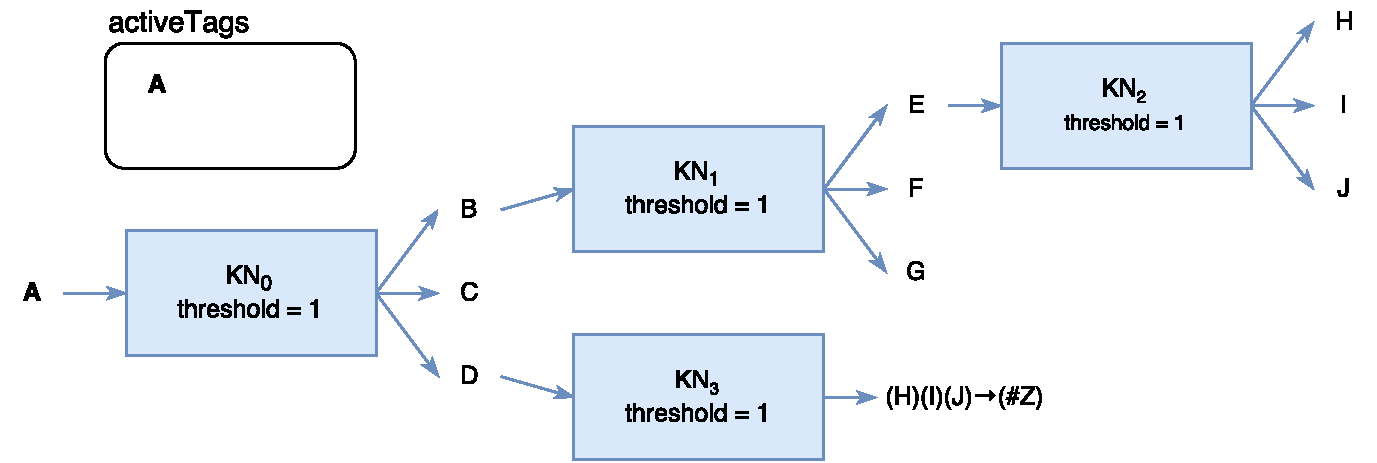
\includegraphics[width=\textwidth]{figures/testKNN.pdf}
\caption[Setup for the \code{testKNN()} method.]
{Initial setup for the \code{testKNN()} method.}
\label{testKNN}
\end{figure*}

\begin{table*}[!htb]
\large
\centering
\begin{tabular}{c | c | c | c | c} 
	\textbf{State} & \textbf{Ready Rules} & \textbf{Active Rules} & \specialcell{\textbf{Active} \\ \textbf{Facts}} & \specialcell{\textbf{Active} \\ \textbf{Recommendations}}  \\ \hline
	
	Initial & \specialcell{$(A)(B)\rightarrow(D)$ \\ $(D)(B)\rightarrow(E)$ \\ $(D)(E)\rightarrow(F)$\\ $(G)(A)\rightarrow(H)$ \\ $(E)(F)\rightarrow(\#Z)$} &  & $(A),(B)$ & $(\#X),(\#Y)$ \\ \hline
	
	$\vdots$ & $\vdots$ & $\vdots$ & $\vdots$ & $\vdots$ \\ \hline
	
	Final & $(G)(A)\rightarrow(H)$ & \specialcell{$(A)(B)\rightarrow(D)$ \\ $(D)(B)\rightarrow(E)$ \\ $(D)(E)\rightarrow(F)$ \\ $(E)(F)\rightarrow(\#Z)$} & \specialcell{$(A),(B),$ \\ $(D),(E)$ \\ $(F)$} & $(\#X),(\#Y),(\#Z)$		
\end{tabular}
\caption[Test setup for \code{testES()}.]
{Test setup for \code{testES()}. Middle activation steps omitted.}
\label{testES}
\end{table*}

\begin{table*}[!htb]
\large
\centering
\begin{tabular}{c | c | c | c | c} 
	\textbf{State} & \textbf{Ready Rules} & \textbf{Active Rules} & \specialcell{\textbf{Active} \\ \textbf{Facts}} & \specialcell{\textbf{Active} \\ \textbf{Recommendations}}  \\ \hline
	Initial
	&$(H)(I)(J)\rightarrow(\#Z)$
	& 
	& \specialcell{$(B),(C),(D)$ \\ $(E),(F),(G)$ \\ $(H),(I),(J)$}
	& \\ \hline
	
	Final
	&
	& $(H)(I)(J)\rightarrow(\#Z)$
	& \specialcell{$(B),(C),(D)$ \\ $(E),(F),(G)$ \\ $(H),(I),(J)$}
	& $(\#Z)$
\end{tabular}
\caption{Test setup and activation for the ES portion of \code{testKNNandES()}.}
\label{testKNNandES}
\end{table*}

\subsection{Testing}

All tests on the system were conducted using the TestNG framework in Java, which provides a simple and intuitive way to create assertions in tests. These tests were placed in the \code{test} package of the project. A UML diagram of the \code{test} package can be seen in \autoref{uml_test} of the Appendix. The primary methods of interest in the test package are \code{testKNN()}, \code{testES()}, and \code{testKNNandES()}.

The test setup for the \code{testKNN()} method can be seen in \autoref{testKNN}. It creates a KNN, with every node having a \code{threshold} value of 1 to simplify the activation process. The system starts out with $A$ as the only active \code{Tag}, and \code{testKNN()} will make the KNN \code{think()} until natural quiescence. It is therefore expected all the \code{Tags} shown in \autoref{testKNN} to become active at the end. The initial and final states are both asserted with TestNG in \code{testKNN()}, with positive results.

The test setup for the \code{testES()} method can be seen in \autoref{testES}. The columns from left to right correspond to the elements in the \code{readyRules}, the \code{activeRules}, the \code{facts}, and the \code{recommendations} respectively. The first row corresponds to the initial setup of the ES, and the last row corresponds to the expected final state. Both the initial and final states are asserted with TestNG in \code{testES()}, with positive results.

The \code{testKNNandES()} method has the same setup as \code{testKNN()} in \autoref{testKNN}, except the output active Tags from the KNN are passed on to the ES. The resulting setup and activation in the ES can be seen in \autoref{testKNNandES}. The initial and final states were also tested with TestNG with positive results.

\subsection{Documentation}

Proper documentation of the source code is very important. This is to ensure that anyone wanting to work with the code which was designed has an easy time doing so. Also, for anyone wanting to understand how the system works, documentation is essential. This documentation was achieved through Javadoc\footnote{The Javadoc can be found here: \url{http://cs.mcgill.ca/~sstapp/prometheus/index.html}} and UML diagrams (see \autoref{sec:uml}).


\section{Plan for Next Semester}
\label{sec:plan}
% In this section you should describe a plan for next semester. What tasks remain to be done, and what is the timeline for accomplishing these tasks? Furthermore you can describe how you plan to test your design in order to make sure it meets the desired specifications. Also outline the design decisions that are required in order to make sure that the final product can be tested.

The plan for next semester is to finalize the two layers that were started this semester (KNN and ES), integrate these layers with the remaining two layers (NN and META), and to test the system in simulation and on the robots available in Prof. Vybihal's lab. The expected timeline can be seen in \autoref{fig:schedule}.

\begin{figure}[!htb]
	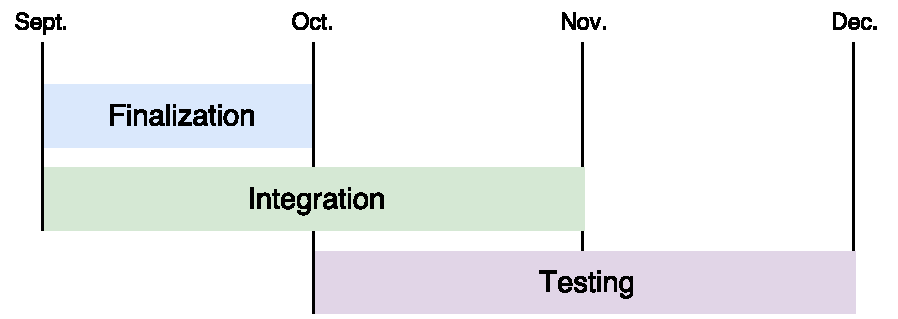
\includegraphics[width=\columnwidth]{figures/schedule.pdf}
	\caption
	{Fall 2017 timeline.}
	\label{fig:schedule}
\end{figure}

\subsection{Finalization}

First, the KNN and ES will need to be finalized. It is expected that this will take up the first month of next semester.

\subsubsection{Knowledge Node Network}

Many features of the KNN layer are still to be implemented, such as backwards and lambda thinking, confidence, and aging.

Backwards thinking can be implemented using a background thread in Java, constantly running in the background at some rate.

Some thought still needs to be put into the specifics on implementation of lambda thinking. Most specifically, there will have to some scoring method to determine how far to search backwards before moving forwards.

Confidence will have to be implemented. Confidence values will probably be associated with every individual \code{Tag}, as well as in an absolute sense in the KNN. Activation through the layers of the KNN can theoretically then reduce the confidence that the output \code{Tags} are true, since at every step the confidence should be multiplied with the previous value.

Aging is also still left to be implemented, with a timestamp system as described in \autoref{sec:background}.

Activation of KNs with sigmoid functions will also be looked into. This can be easily implemented using a cache of known sigmoid values.

Also, more thought will have to be put into the design of the KNN to allow cyclic graphs, representing recursive memories in the human brain.

Finally, there will be more features to be added in the KNN which are not described in \autoref{sec:background}, since they are still in the process of being thought out. These features include learning, long-term memory and attention.

\subsubsection{Expert System}

Some features of the ES layer are still to be implemented, such as more complex \code{Fact} checking. Indeed, currently, the ES only checks for strict equality between \code{Facts}, but it would be interesting to implement checking for ``greater than" or ``less than" relations as well.

\subsection{Integration}

One very important task left to be done is to integrate the two layers described in this report (ES and KNN) with the other layers developed separately (NN and META). Ideally, the layers should be able to work together, but there will surely be some conflicts at the interface of the layers. These will have to be resolved when the time comes.

The interface between the NN and the KNN will have to be tested. There may have to be some conversion between what the NN will output and what the KNN expects (\code{Tags}). The META layer is also still to be implemented. It is crucial, since it will decide the way the KNN will think.

The integration section is expected to take around 2 months, with the the first month overlapping with the finalization section.

\subsection{Testing}

Finally, the system will have to be tested. This is expected to take around 2 months, with the first month overlapping with the last month of integration.

The first and easiest way to test would be in a simulated environment. One simulator that may be used is Simbad, which is a Java 3D robot simulator \cite{simbad}. This can allow for some early debugging and fixes.

Once the simulation testing is completed and working properly, the system can be tested in the lab. Prof. Vybihal's lab has multiple robots with ultrasonic sensors, and these will be the test subjects of this phase.

\section{Impact on Society and the Environment}
% In one or two pages, discuss the environmental and/or social impact of your project. Your analysis should include your work at McGill as part of this project, however, the main focus should be on the product/system you are designing (e.g., the cost/benefit/risk of manufacturing it, the cost/benefit/risk for consumers using it) or the problem your thesis is addressing (e.g., how will solving the problem influence/affect/benefit society and the environment). Particular emphasis should be given to:


\subsection{Use of Non-renewable Resources}
% Consider all stages of the product from design, manufacturing, distribution, use by consumers, and disposal/recycling.

As purely a software project, there are no physical materials needed to construct this system. For this reason, less emphasis will be put on this section. The only physical resources potentially needed are the materials needed to construct the robots and the computers to house the software. One area of concern could be the energy source of the robots themselves, which would probably vary depending on context. Ideally, the source should be a renewable one. For example, solar panels could be placed on the robots to provide energy.

\subsection{Environmental Benefits}
% Benefits to the environment, comparisons with more polluting technologies etc.

Prometheus could be used in a context beneficial to the environment. For example, the system could be used as a tool to control robots after oil spills, where the robots could theoretically contain the problem faster than humans and thus limit the risk on the environment. There is already research being done on employing robots in this context. Indeed, MIT's Senseable City Lab has been working on Seaswarm, a system composed of a fleet of vehicles to help clean future oil spills \cite{seaswarm}. An AI like Prometheus to control a swarm of robots like this could be very valuable. 

\subsection{Safety and Risk}
% To you undertaking the project, as well as to any potential users of the solution once it is finished.

It is critical that, once this system is completed, it is used in an ethical way, and for the right purposes. One example of use that may cause ethical concern is in a military setting, where an AI system like the one described here could be used in a battlefield in place of soldiers. Indeed, the US Department of Defense has plans to employ AI for autonomous weapons to attack targets without human intervention in the future \cite{military}. This would have the advantage of potentially saving human soldiers' lives \cite{define_military_ai}. However, there are also concerns because this would make it much easier to start a battle. More than 3000 AI and robotics researchers have signed an open letter arguing against a military AI arms race \cite{openletter}. They argue that autonomous weapons would not be beneficial to society, since they would be ideal for assassinations, destabilizing countries or selectively subduing or killing a population.

Another possible issue is the future loss of jobs to be done by humans, with automated systems like Prometheus replacing physical labor. This problem can be solved as a society, perhaps by having more support for universal basic income (UBI). Telsa CEO Elon Musk is a proponent of the idea, saying that UBI will be necessary in the future \cite{musk}. Bill Gates suggests possibly having a tax on robots to help pay for this income \cite{gates}.

In the very long term, there are concerns with the possibility that an AI system might achieve intelligence and awareness close to a human. If such an AI were to obtain ``consciousness'' in its own way, should that entity be entitled to its own rights, like humans or animals are? The issue has been mentioned by the Institute for the Future, calling for the possibility of ``robo-rights'' in the future \cite{robo_rights}.


% TODO: Reorganize society with high-level thinking, common salary

\subsection{Benefits to Society}
% Quality of life, economic benefits, etc.

This type of system could be extremely useful in many contexts in society. For instance, the system could be used to send and control robots in an area that would otherwise be very dangerous for humans. For example, robots are often used in the aftermath of nuclear disasters to prevent the unnecessary loss of human life. Indeed, even in the Chernobyl nuclear disaster, the Soviet authorities employed the use of robots to avoid losses of human life \cite{chernobyl}. With an AI like Prometheus, the robots could be controlled in an intelligent manner.

The system could also be used to further space exploration, with an AI controlling multiple robots exploring the surface of Mars, for instance. The value of AI in this context has been clearly shown, with the Mars Curiosity rover recently being upgraded to have its own AI system using computer vision to identify rocks \cite{rover}. This system can therefore help further important cutting-edge research in space exploration.

\section{Conclusion}
% Use this section to summarize what was accomplished in this semester, provide a summary of the next steps and share any insight you have learned.

This semester, prototypes of the Expert System (ES) and Knowledge Node Network (KNN) layers of the Prometheus AI model were completed in Java based on personal design criteria and feedback from the supervisor. The design of the prototypes has required a great deal of thought and planning to ensure efficiency and proper behaviour. These prototypes were tested using the TestNG Java framework with positive results, and extensive Javadoc was produced.

The main goal for next semester is to finalize the entire system, implementing more complex features that were omitted for this prototype stage. This will also require proper integration between the work done in this report (KNN and ES), and outside this report (NN and META). Finally, the entire system will have to be tested, in simulation and with physical robots.

\clearpage
\onecolumn
\appendix

\renewcommand\thefigure{\thesection.\arabic{figure}}
\setcounter{figure}{0}    

\section{UML Diagrams}
\label{sec:uml}
% TODO: update UML diagrams

\begin{figure}[!htb]
	\centering
	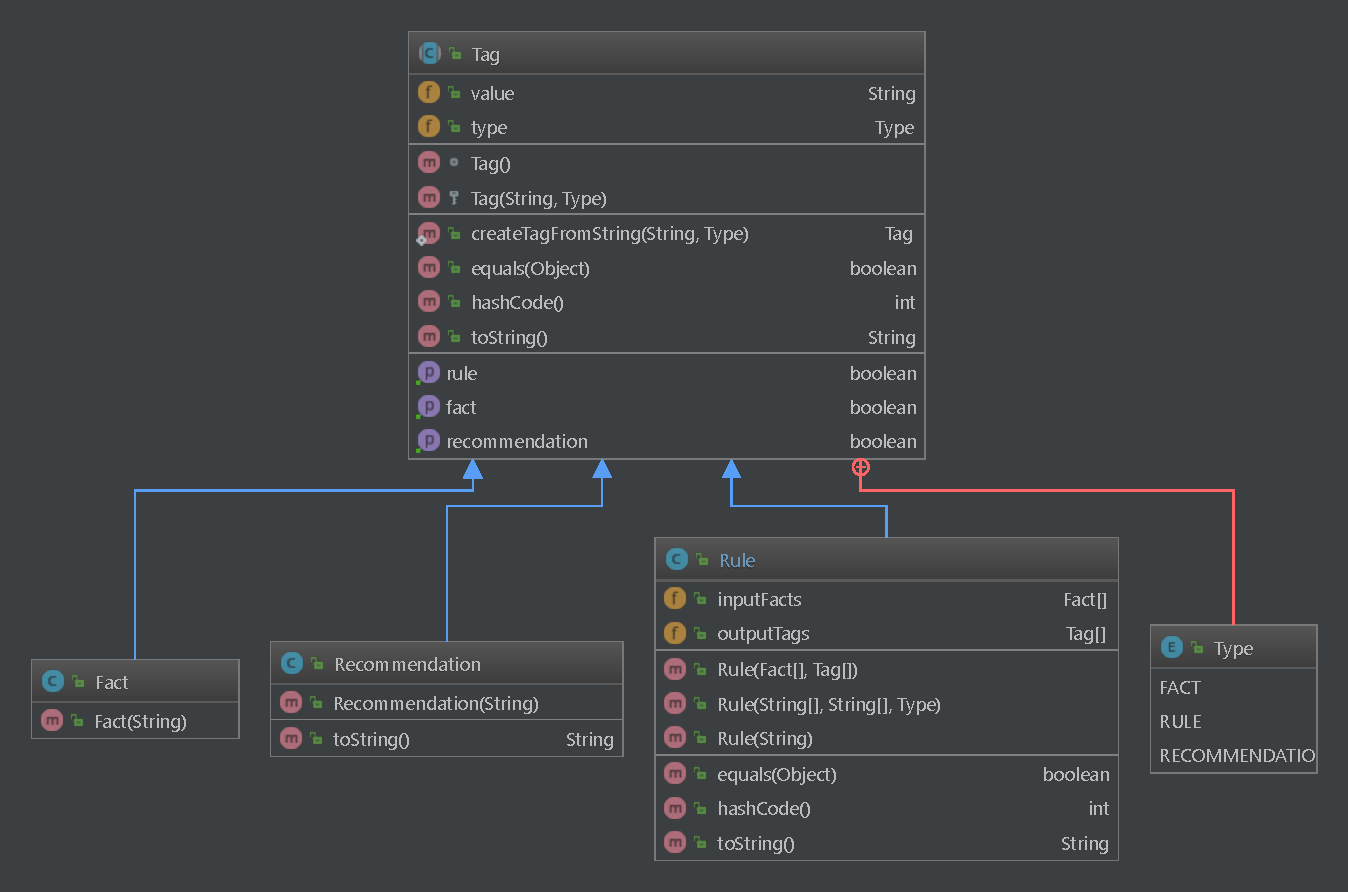
\includegraphics[width=\columnwidth]{figures/uml_tags.pdf}
	\caption{UML diagram of the \code{tags} package.}
	\label{uml_tags}
\end{figure}

\begin{figure}[!htb]
	\centering
	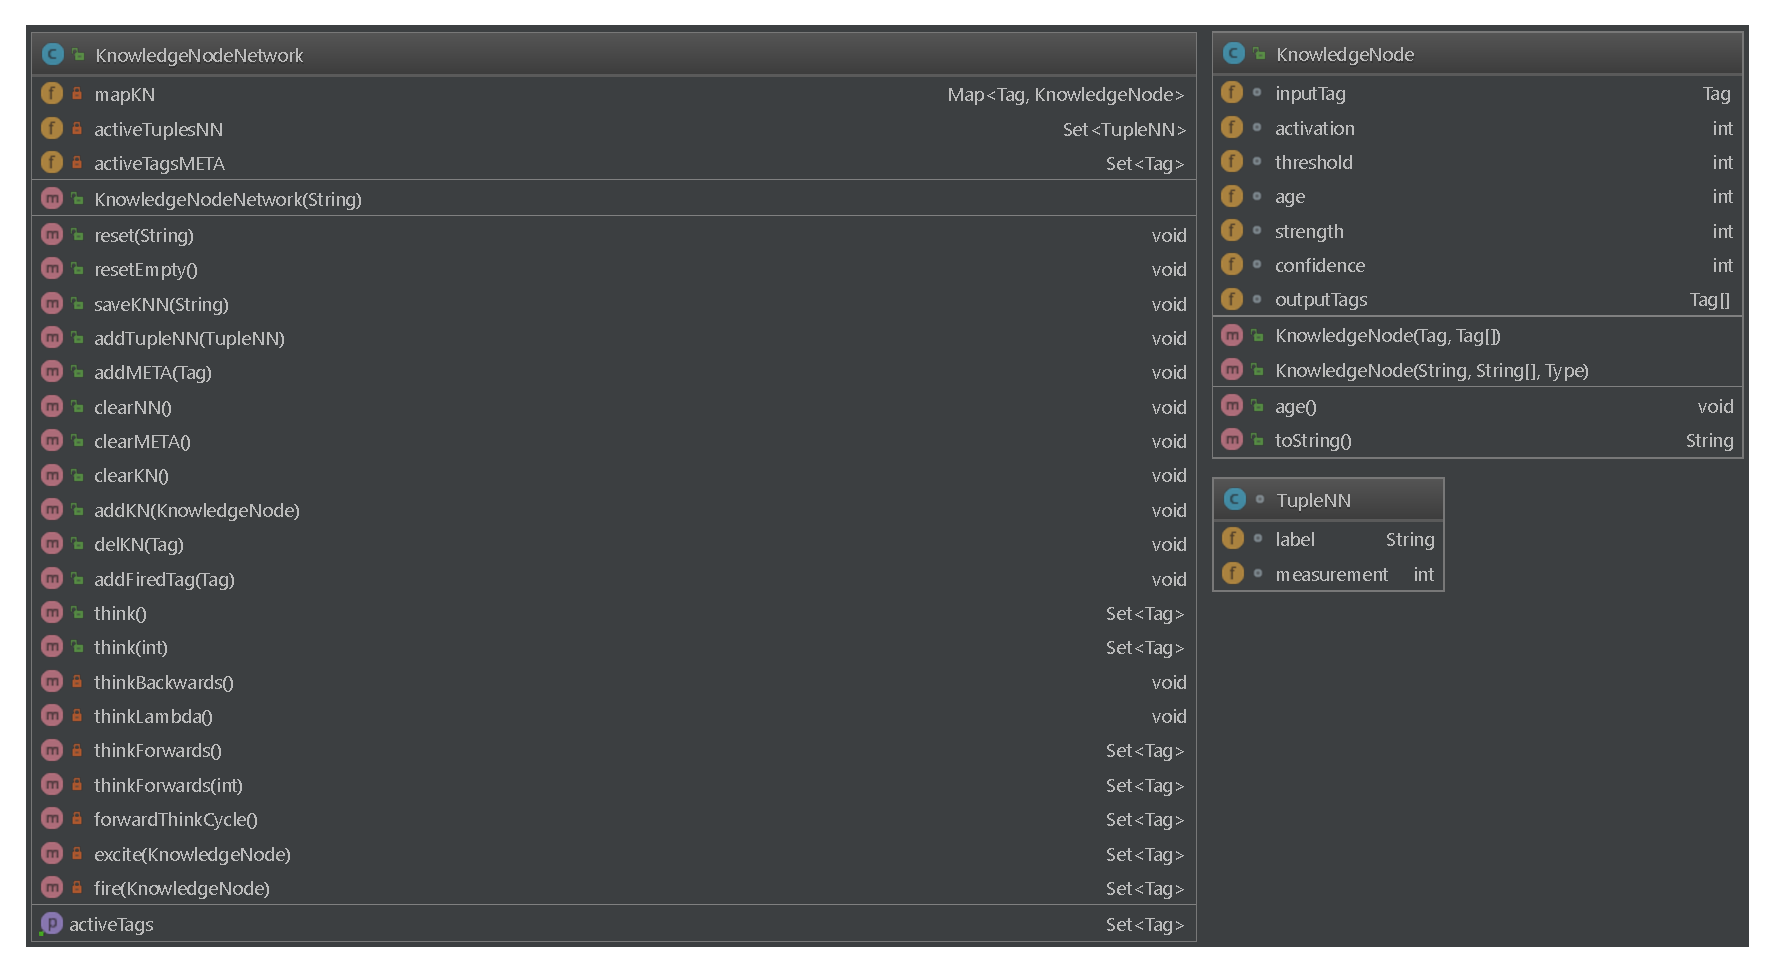
\includegraphics[width=\columnwidth]{figures/uml_knn.pdf}
	\caption{UML diagram of the \code{knn} package.}
	\label{uml_knn}
\end{figure}

\begin{figure}[!htb]
	\centering
	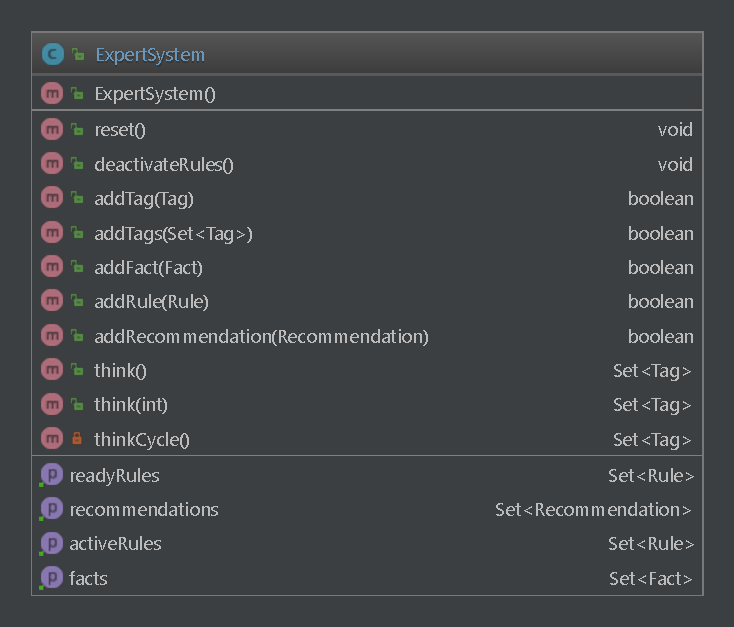
\includegraphics[width=0.5\columnwidth]{figures/uml_es.pdf}
	\caption{UML diagram of the \code{es} package.}
	\label{uml_es}
\end{figure}

\begin{figure}[!htb]
	\centering
	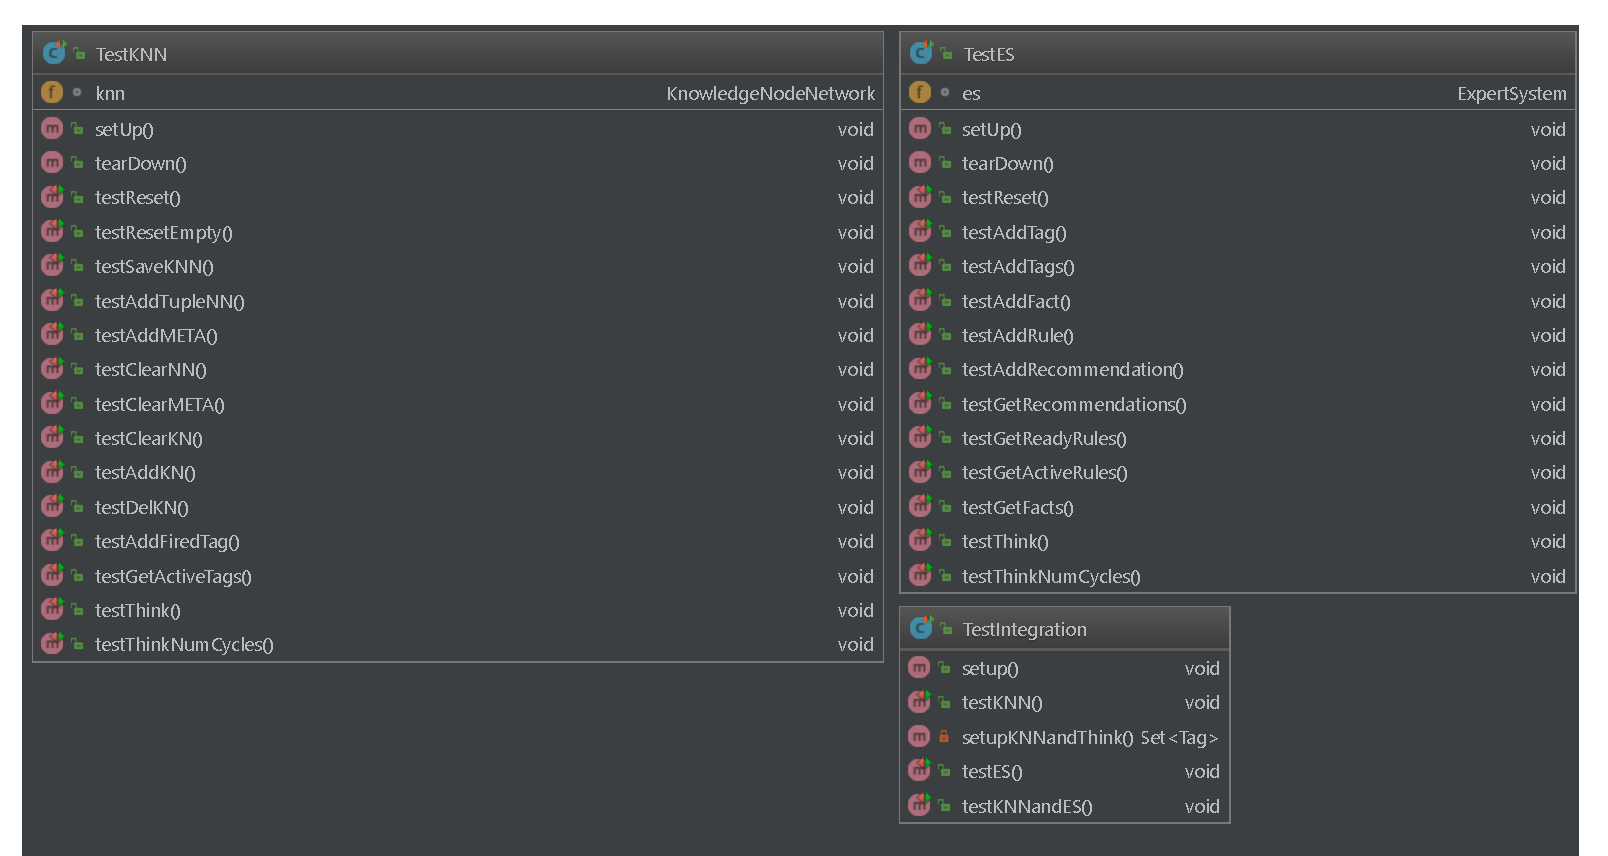
\includegraphics[width=\columnwidth]{figures/uml_test.pdf}
	\caption{UML diagram of the \code{test} package.}
	\label{uml_test}
\end{figure}

\clearpage

\bibliography{readings}{}
\bibliographystyle{IEEEtran}

\end{document}